\setcounter{chapter}{-1} % make this chapter 0
\chapter{Introduction}
%\addcontentsline{toc}{chapter}{Introduction} % but still display in TOC (see https://tex.stackexchange.com/a/222961)

%Inspiration
%\url{https://en.wikipedia.org/wiki/White_dwarf#Formation}
%\url{https://en.wikipedia.org/wiki/Compact_star}

Ever since the dawn of mankind, humans have gazed upon the night sky with great curiosity of what lies beyond our reach and how it all fits together with our existence.
During the 20th century, physicists have developed two irreplaceable tools for understanding its structure -- general relativity by Einstein and quantum theory by numerous physicists.
The most exotic type of star currently known to man is neutron stars, formed in the supernova explosion of massive stars that are not massive enough to collapse into black holes.
In this thesis, we are going to study the fundamentals of neutron stars, from the theory of general relativity to their equation of state by quantum field theory.

\section{The life and death of stars}

\begin{figure}
\centering
\usetikzlibrary{positioning}
\usetikzlibrary{shapes.symbols}
\usetikzlibrary{shadows}
\usetikzlibrary{trees}
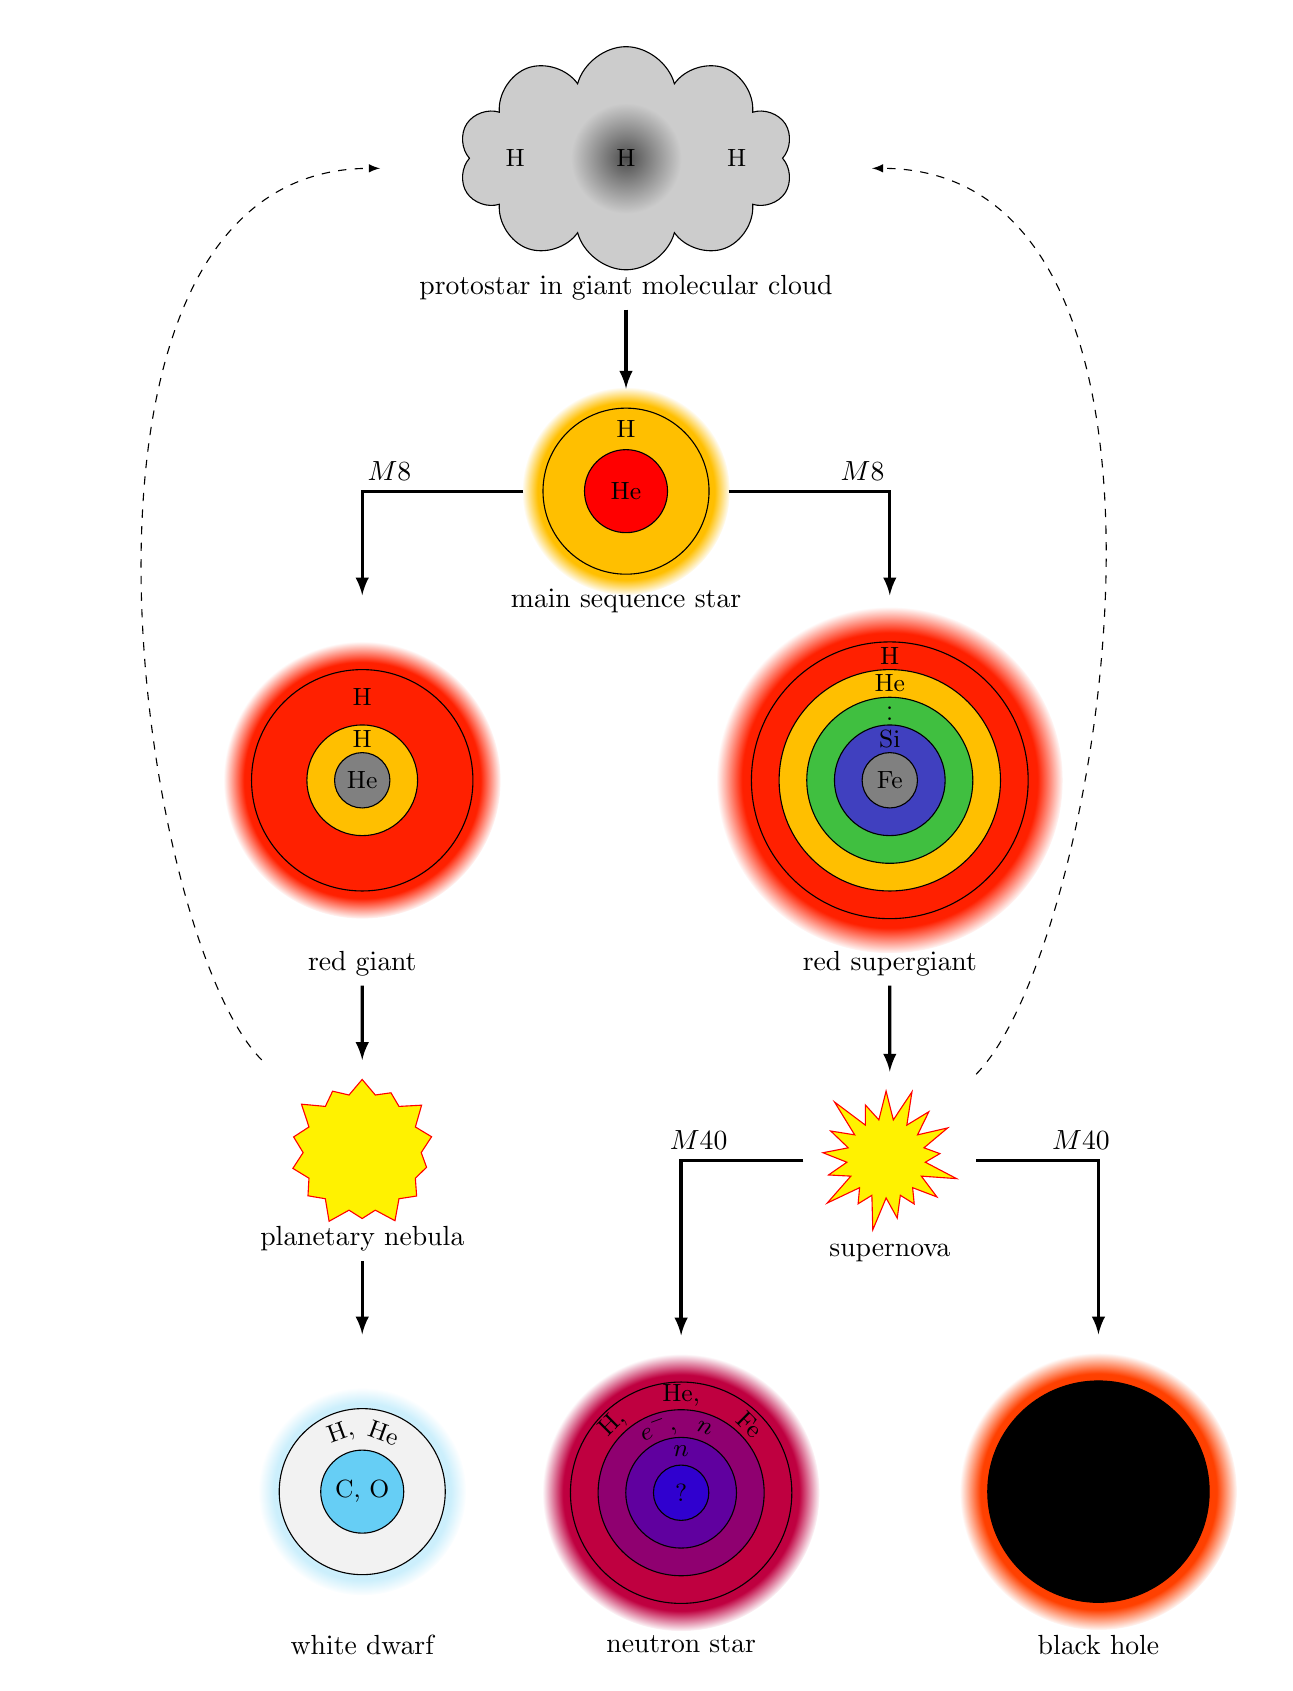
\begin{tikzpicture}[
	edge from parent/.style={draw,very thick,-latex},
	level distance=5cm,
	level 1/.style={level distance=4.1cm},
	level 2/.style={level distance=3.8cm, sibling distance=6.7cm},
	level 3/.style={level distance=4.7cm},
	level 4/.style={level distance=4.3cm, sibling distance=5.3cm},
	sibling distance=6cm,
	every label/.style={text width=4cm, text centered, inner sep=0pt, yshift=+2pt},
	element/.style={font=\small},
	dualpath/.style={
		edge from parent path={(\tikzparentnode\tikzparentanchor) -| (\tikzchildnode\tikzchildanchor)},
	},
	cloud/.pic={
		\node [draw, cloud, element, aspect=2, fill=gray, inner sep=10pt] {H};
	},
	protostar/.pic={
		\node [draw, cloud, aspect=2, fill=black!20!white, inner sep=20pt] {};
		\shade [even odd rule, inner color=black!70!white, outer color=black!20!white] circle (20pt);
		\node [element] at (0, 0) {H};
		\node [element] at (-40pt, 0) {H};
		\node [element] at (+40pt, 0) {H};
	},
	mainsequencestar/.pic={
		\draw[draw=black, fill=orange!50!yellow, circular glow={fill=orange!50!yellow}] circle [radius=30pt]; \node [element] at (90:22.5pt) {H};
		\draw[draw=black, fill=red] circle [radius=15pt]; \node [element] at (90:0pt) {He};
	},
	browndwarf/.pic={
		\filldraw[brown] circle [radius=20pt];
		\node [element] at (90:0pt) {H};
	},
	redgiant/.pic={
		\draw[draw=black, fill=red!75!orange, circular glow={fill=red!75!orange}] circle [radius=40pt]; \node [element] at (90:30pt) {H};
		\draw[draw=black, fill=orange!50!yellow] circle [radius=20pt]; \node [element] at (90:15pt) {H};
		\draw[draw=black, fill=gray] circle [radius=10pt]; \node [element] at (90: 0pt) {He};
		\draw[draw=none] (-60pt,-60pt) rectangle (+60pt,+60pt);
	},
	redsupergiant/.pic={
		\draw[draw=black, fill=red!75!orange, circular glow={fill=red!75!orange}] circle [radius=50pt]; \node [element] at (90:45pt) {H};
		\draw[draw=black, fill=orange!50!yellow] circle [radius=40pt]; \node [element] at (90:35pt) {He};
		\draw[draw=black, fill=green!50!gray] circle [radius=30pt]; \node [element] at (90:25pt) {$\vdots$ };
		\draw[draw=black, fill=blue!50!gray] circle [radius=20pt]; \node [element] at (90:15pt) {Si};
		\draw[draw=black, fill=gray] circle [radius=10pt]; \node [element] at (90:0pt) {Fe};
		\draw[draw=none] (-60pt,-60pt) rectangle (+60pt,+60pt);
	},
	supernova/.pic={
		\node[starburst, fill=yellow, draw=red, minimum size=2cm] {};
	},
	planetarynebula/.pic={
		\node[starburst, starburst points=14, starburst point height=0.25cm, fill=yellow, draw=red,  minimum size=2.0cm] {};
	},
	blackhole/.pic={
		\draw [fill=black, circular glow={fill=red!50!orange}] circle[radius=40pt];
		\draw[draw=none] (-50pt, -50pt) rectangle (+50pt, +50pt);
	},
	neutronstar/.pic={
		\draw[draw=black, fill=blue!  0!purple, circular glow={fill=blue!0!purple}] circle [radius=40pt]; \node [element, rotate=45] at (135:35pt) {H,}; \node [element] at ( 90:35pt) {He,}; \node [element, rotate=-45] at (45:35pt) {Fe};
		\draw[draw=black, fill=blue! 25!purple] circle [radius=30pt]; \node [element, rotate=+20] at (110:25pt) {$e^-$,}; \node [element, rotate=-20] at (70:25pt) {$n$};
		\draw[draw=black, fill=blue! 50!purple] circle [radius=20pt]; \node [element] at (90:15pt) {$n$};
		\draw[draw=black, fill=blue! 75!purple] circle [radius=10pt]; \node [element] at (90: 0pt) {?};
		\draw[draw=none] (-50pt, -50pt) rectangle (+50pt, +50pt);
	},
	whitedwarf/.pic={
		\draw[draw=black, fill=white! 90!gray, circular glow={fill=cyan! 20!white}] circle [radius=30pt]; \node [element, rotate=+20] at (110:22.5pt) {H,}; \node [element, rotate=-20] at (70:22.5pt) {He};
		\draw[draw=black, fill=cyan! 60!white] circle [radius=15pt]; \node [element] at (90:0pt) {C, O};
		\draw[draw=none] (-50pt, -50pt) rectangle (+50pt, +50pt);
	},
]

	\node (protostar) {\tikz \node [label={[text width=6.0cm]below:\subcaption{\label{fig:intro:star_evolution_protostar}protostar in giant molecular cloud}}] {\tikz \pic {protostar};};}
		child { node [label={[]below:\subcaption{\label{fig:intro:star_evolution_mainseq}main sequence star}}] {\tikz \node [] {\tikz \pic {mainsequencestar};};}
			child { node {\tikz \node [label={below:\subcaption{\label{fig:intro:star_evolution_red_giant}red giant}}] {\tikz \pic {redgiant};};}
				child { node (planetarynebula) {\tikz \node [label={below:\subcaption{\label{fig:intro:star_evolution_planetary_nebula}planetary nebula}}] {\tikz \pic {planetarynebula};};}
					child { node {\tikz \node [label={below:\subcaption{\label{fig:intro:star_evolution_white_dwarf}white dwarf}}] {\tikz \pic {whitedwarf};};} }
				} edge from parent [dualpath] node [above, anchor=south west, xshift=-2pt] {$M \lesssim 8 \solarmass$}
			}
			child { node {\tikz \node [label={below:\subcaption{\label{fig:intro:star_evolution_red_supergiant}red supergiant}}] {\tikz \pic {redsupergiant};};}
				child { node (supernova) [label={below:\subcaption{\label{fig:intro:star_evolution_supernova}supernova}}] {\tikz \node [] {\tikz \pic {supernova};};}
					child { node {\tikz \node [label={below:\subcaption{\label{fig:intro:star_evolution_neutron_star}neutron star}}] {\tikz \pic {neutronstar};};} edge from parent [dualpath] node[above, anchor=south west, xshift=-8pt] {$M \lesssim 40 \solarmass$} }
					child { node {\tikz \node [label={below:\subcaption{\label{fig:intro:star_evolution_black_hole}black hole}}] {\tikz \pic {blackhole};};} edge from parent [dualpath] node[above, anchor=south east, xshift=+8pt] {$M \gtrsim 40 \solarmass$} }
				}
				edge from parent [dualpath] node [above, anchor=south east, xshift=+2pt] {$M \gtrsim 8 \solarmass$}
			}
		};
	\draw [-latex, dashed] (supernova)       to [out= 45, in=  0, out looseness=0.5] (protostar);
	\draw [-latex, dashed] (planetarynebula) to [out=135, in=180, out looseness=0.5] (protostar);
\end{tikzpicture}
\caption{\label{fig:intro:star_evolution}%
	Simplified life cycle of stars and their main structure at every stage (not to scale).
}
\end{figure}

% planetary nebula -> releases ionized gas -> forms clouds
The mother of any star is an enormous accumulation of light elements like hydrogen called a \textbf{giant molecular cloud}, formed by the ashes of dying stars at the end of the life cycle we have just begun to describe.
Such clouds consist of matter weighing up to tens of millions solar masses, distributed with a relatively low average density over a huge area that up to hundreds of lightyears across.
Internally, the dynamics of a molecular cloud is chiefly governed by the attractive force of gravity between particles and the repulsive thermal pressure from their motion and collisions.

Due to the force of gravity, parts of the cloud can clump together in areas of greater density.
As more mass accumulates, the force of gravity attracting the surrounding material only increases, causing a snowball effect that only amplifies the growth of the clump.
Initially, the material is not so dense, and thermal radiation can escape outside, causing low temperatures and pressure and allowing the clump to contract with little resistance.
However, once the density becomes sufficiently high, thermal radiation can no longer find its way out and is trapped inside.
When this happens, the temperature increases, in turn increasing the outwards pressure that counteracts the inwards gravitational collapse and considerably slows down the contraction.
During this stage depicted in \cref{fig:intro:star_evolution_protostar}, as the child ``clump'' grows by sucking up material from its parent cloud, it receives the more honorable name \textbf{protostar}.

Sooner or later, the protostar has depleted the cloud of its available mass.
It then continues to contract, causing the temperature and pressure to increase, ultimately reaching a state of equilibrium with the gravitational collapse.
The protostar is then promoted to a \textbf{main sequence star}.
Provided that the protostar has accumulated at least $M \gtrsim 0.08 \solarmass$, the temperature will reach $T \gtrsim \SI{1e7}{\kelvin}$ -- sufficient for the fusion of hydrogen into helium to take place.
For billions of years, the star supports itself by burning hydrogen into helium.
The heavier helium is pulled into the central regions of the star, establishing a helium \emph{core} surrounded by an \emph{envelope} constisting of the lighter hydrogen, as shown in \cref{fig:intro:star_evolution_mainseq}.

What happens after most of the hydrogen has burnt up depends heavily on the mass of the star.
Stars up to $M \lesssim 8 \solarmass$ evolve into \textbf{red giants}.
As the hydrogen fails to support the star, the core begins to contract again.
For heavier red giants, the temperature can increase to $T \gtrsim \SI{1e8}{\kelvin}$, activating both fusion of helium to carbon and carbon to oxygen, but the temperature is too low for fusion of heavier elements.
The core develops shells with elements of increasing weight towards the center as shown in \cref{fig:intro:star_evolution_red_giant}, from hydrogen to helium, carbon, or oxygen, depending on the exact mass of the star.
Due to the sudden increase in temperature, much energy is transported into the envelope, where it ignites leftover hydrogen and inflates the envelope up to 200 solar radii -- hence the name of the star.

Eventually, explosions in the envelope of a red giant trigger unstable pulsations of the hydrogen envelope.
This causes a \textbf{planetary nebula}, depicted in \cref{fig:intro:star_evolution_planetary_nebula} -- an ejection of the outer shells of the red giant into new interstellar clouds from which new starts can be born at a restart of the cycle.
The remaining inert core that is intact from the nebula forms a \textbf{white dwarf}.
Illustrated in \cref{fig:intro:star_evolution_white_dwarf}, a white dwarf is essentially the core of the preceeding red giant that is intact after the planetary nebula.
Since no further reactions occur, it is supported against collapse solely by electron degeneracy pressure.
White dwarves can be as hot as $T \approx \SI{1e7}{\kelvin}$ upon formation, but gradually cool down as they radiate away their energy.
Importantly, white dwarves can only support themselves for masses up to the Chandrasekhar limit $M \lesssim 1.4 \solarmass$.
\TODO{cooling etc}

If the mass of a main sequence star exceeds $M \gtrsim 8 \solarmass$, it essentially becomes a more dramatic a red giant -- namely a \textbf{red supergiant}.
The increased mass sends the temperature soaring well above $T \gtrsim \SI{1e8}{\kelvin}$, activating not only fusion from hydrogen to helium, carbon and oxygen, but even fusion to heavier elements such as neon and iron.
When the reactions reach iron, something dramatic happens.
In contrast to elements lighter than iron, fusion from iron or heavier elements \emph{require} energy instead of releasing it.
The burning therefore stops at iron.
At this point, the core of a red supergiant is so massive due to the more massive elements that it exceeds the Chandrasekhar limit.
Thus, the core collapses in an explosion called a \textbf{supernova}, illustrated in \cref{fig:intro:star_evolution_supernova}.
\TODO{iron peak graph?}

For supergiants whose mass does not exceed $M \lesssim 40 \solarmass$, the core left behind by the supernova is called a \textbf{neutron star}.
The core collapse of the supergiant has compressed the core past the white dwarf stage, reaching a new equilibrium composition of neutrons, protons, hyperons, leptons and possibly quarks.
Like white dwarves, neutron stars are ovens that are burnt out, and only continue to cool down and shine.
\TODO{temperature? new 1e11-1e12 K, quickly decays to 1e6, then radiate away and cool down}

Even more massive supergiants with more than $M \gtrsim 40 \solarmass$ experience such a tremendous force of gravity that they collapse directly to \textbf{black holes}, depicted in \cref{fig:intro:star_evolution_black_hole}.

\section{From proposition to observation and theory of neutron stars}

Only two years after James Chadwick discovered the neutron in 1932, \cite{ref:neutron_discovery}
Walter Baade and Fritz Zwicky proposed the existence of stars composed of this particle. \cite{ref:supernova_cosmic_rays_neutron_stars}
First, they proposed that supernovae -- which scientists had just begun to study -- was the origin of cosmic rays -- energetic streams of protons and atomic nuclei moving through space.
In developing an explanation of the detailed mechanisms involved in this process, Baade and Zwicky simultaneously suggested -- with great accuracy -- that
\begin{displayquote}
(...) %With all reserve we advance the view that
a super-nova represents the transition of an ordinary star into a neutron star, consisting mainly of neutrons.
Such a star may possess a very small radius and an extremely high density.
As neutrons can be packed much more closely than ordinary nuclei and electrons, the "gravitational packing" energy in a cold neutron star may become very large, and, under certain circumstances, may far exceed the ordinary nuclear packing fractions.
A neutron star would therefore represent the most stable configuration of matter as such.
\cite[page 263]{ref:supernova_cosmic_rays_neutron_stars}
\end{displayquote}
Today, it is known that supernovae do indeed account for most cosmic rays, and that they do indeed mark the transition of an ordinary star into neutron stars or black holes.

The first theoretical model of a neutron star was developed by Oppenheimer and Volkoff in 1939. \cite{ref:tov}
Assuming a neutron star consists entirely of a non-interacting cold Fermi gas, they found an equation of state governing its internals and solved the Einstein field equations in a radially symmetric perfect fluid to find the mass and radii of neutron stars.
In such a cold gas, thermal motion contributes nothing to the pressure, so any pressure is only due to the Pauli exclusion principle, stating that no fermions can be in the same quantum state.
Analogously to the Chandrasekhar limit, their results implied that this degeneracy pressure could only support masses up to $M < 0.7 \solarmass$.

Assuming a neutron star consists entirely of a free and cold Fermi gas, Oppenheimer and Volkoff in 1939 predicted \TODO{?} that the mass of a neutron star cannot exceed $M < 0.75 \solarmass$ \cite{ref:tov} -- a limit analogous to the Chandrasekhar limit for white dwarves.

% see https://en.wikipedia.org/wiki/Pulsar
Up until the late 1960s, the existence of neutron stars was only considered a theoretical possibility.
Given their small size, assumed rarity and faint thermal radiation, experimentalists did not have much of a clue how one would observe them.
It was first in 1968 that Jocelyn Bell, a PhD student supervised by A?? Hewish, recorded an unusual \textbf{pulsa}ting \textbf{r}adio signal from an extraterrestial source, now referred to as a \textbf{pulsar}. \cite{ref:neutron_star_discovery_first}
The signal consisteded of short, Gaussian pulses lasting about \SI{0.3}{\second} that repeated with extreme accuracy with a period of \SI{1.337}{\second}. \TODO{show plot in figure?}
At first, it was speculated that the source could be a white dwarf oscillating radially at this frequency.
Thomas Gold provided an alternative explanation, suggesting the signal arose from a rotating neutron star with a strong magnetic field. \cite{ref:neutron_star_gold}
He thought the star's magnetic field to be reminiscent of a dipole and that the signal was emitted from localized spots on the star corresponding to the magnetic poles.
This picture naturally explained the Gaussian shape of the short pulses, just like the beam from a rotating lighthouse flashing an observer at night.
In contrast, radial pulsations did not explain the shape nor the extreme regularity of the signal.
Not long after, Richard Lovelace and others measured a similar signal from the pulsar NP 0532 in the Crab Nebula -- also referred to as the Crab Pulsar -- with a period of only \SI{33}{\milli\second}, which could not be explained by radial oscillations. \cite{ref:crab_pulsar_period_discovery}
Moreover, D.W. Richards discovered that the period seemed to increase, as it should for a rotating object that radiates away energy.
This development convinced physicists that the signals were indeed from real, rotating and pulsating \textbf{neutron stars}.
Controversially, Bell's supervisor Hewish and Martin Ryle later got the Nobel prize for their first discovery of a neutron star, although it is Jocelyn who made the actual measurements and is usually credited in hindsight.


% see https://en.wikipedia.org/wiki/Tolman%E2%80%93Oppenheimer%E2%80%93Volkoff_limit
To this day, many neutron stars have been discovered with mass up to X has been observed, showing that the Oppenheimer-Volkoff limit is wrong.
Modern, advanced theories take into account that a neutron star consists not only of neutrons, but also of other particles.
We return to this question in the conclusion and outlook.



Since the dawn of mankind, humans have gazed upon the night sky with great curiosity of what lies out in the universe.
\begin{itemize}
\item Establish the importance of studying stars from an existential point of view.
\item Give a brief historical review of how our view of stars and the universe has changed, from the nonscientific views of the earliest days to the scientific viewpoint of the modern age.
\end{itemize}

After the discovery of the neutron in 1933, scientists soon proposed the existence of stars consisting of neutrons.
\begin{itemize}
\item Explain why neutron stars are plausible, from the original ``ignorant'' point of view before one has a good theoretical understanding of neutron stars.
\item Review the hypotheses that came from the initial theoretical work on neutron stars, before any observation was made.
\end{itemize}

In 1967, Jocelyn Bell and Antony Hewish discovered the first known neutron star.
\begin{itemize}
\item Review observations that have been made from neutron stars up until today.
\item Connect the observations made to the theoretical hypotheses from the last paragraph.
\end{itemize}

Today, scientists have a good understanding of neutron stars.
\begin{itemize}
\item Explain the modern, ``perfect'' understanding of neutron stars, that have not been covered by the ``naive'' view in the last two paragraphs.
\item Explain that neutron stars are formed by supernova explosions.
\item Explain that neutron stars are the smallest and densest class of stars that have been observed.
\item Explain that neutron stars are kept stable by the balance between gravitational attraction and Pauli pressure.
\end{itemize}

Being one of the most exotic types of objects humanity has observed, neutron stars are a gateway to developing our understanding of new, hypothetical astronomical objects.
\begin{itemize}
\item Explain why it is important to understand neutron stars first (even if others already understand them), in order to do new and interesting work.
\item Explain the possibility that neutron stars can develop into even more, currently hypothetical classes of stars, such as quark stars.
\end{itemize}

\section{Outline of this thesis}

In this thesis, we first develop the fundamental theoretical tools that are necessary to study neutron stars.
Then we apply them to calculate masses and radii of neutron stars and study the stability of these stars.

In \textbf{\cref{chap:tov}}, we derive the \textbf{Tolman-Oppenheimer-Volkoff system of equations}
\begin{align*}
	\odv{P}{r} &= -\frac{G m \epsilon}{r^2 c^2} \left( 1 + \frac{P}{\epsilon} \right) \left( 1 + \frac{4 \pi r^3 P}{m c^2} \right) \left( 1 - \frac{2 G m}{r c^2} \right)^{-1} , \\
	\odv{m}{r} &= \frac{4 \pi r^2 \epsilon}{c^2} ,
	%\odv{\alpha}{r} &= -\frac{1}{\epsilon(P)+P} \odv{P}{r} ,
\end{align*}
from the Einstein field equations of general relativity.
This is a system of two differential equations for the unknown pressure $P(r)$, mass $m(r)$ and energy density $\epsilon(r)$ at radius $r$ from the center of a star composed of a \emph{perfect fluid} in \emph{equilibrium}.
An additional equation of state $\epsilon = \epsilon(P)$ that allows computation of the energy density corresponding to a given pressure is needed to solve the system.
This is outside the scope of general relativity and belongs to the field of quantum theory and statistical mechanics.
Given the equation of state, however, one may impose the boundary condition $m(0) = 0$ and any central pressure $P(0) = P_0$ and solve the system for the pressure profile $P(r)$ and mass profile $m(r)$ in the star.
By defining the surface $r=R$ of the star where the pressure $P(R) = 0$ vanishes, one can obtain the radius $R$ and mass $M = m(R)$ of the star.
In particular, we will solve the system analytically for a star of constant energy density $\epsilon(P) = \epsilon_0$ to derive the Buchdal limit
\begin{equation*}
	\frac{M}{R} < \frac{4 c^2}{9 G}
\end{equation*}
on the mass-radius ratio of \emph{any} star.

In \textbf{\cref{chap:tft}}, we will study \textbf{thermal field theory} -- the formalism needed to find the effects of quantum fields at nonzero temperature.
We will show how to write the quantum partition function
\begin{equation*}
	Z = \trace \left[ e^{-\beta(\hat{H} - \mu_i \hat{N}_i)} \right]
\end{equation*}
as a path integral.
First, we use the path integral to find the partition function of a gas of free bosons.
Next, we introduce Grassmann numbers and fermionic coherent states to derive a path integral that is valid for fermions, and calculate it for a non-interacting Fermi gas of free Dirac fermions.
From this partition function, we can calculate the energy density and pressure and hence the equation of state.

In \textbf{\cref{chap:nstars}}, we put together the pieces of \cref{chap:tov} and \cref{chap:tft} and study \textbf{neutron stars} made of a \textbf{cold, non-interacting Fermi gas}.
From the partition function $Z$ of \cref{chap:tft}, we find the equation of state
\begin{equation*}
	\epsilon = \epsilon(P)
\end{equation*}
for a cold Fermi gas made of free neutrons.
We then solve the Tolman-Oppenheimer-Volkoff equation numerically for this equation of state to find a mass-radius curve $[R(P_0), \, M(P_0)]$ for such stars parametrized by their central pressure.
Finally, we study whether stars on the curve are in stable or unstable equilibrium.
We begin by establishing a set of necessary criterions from simple physical considerations.
Then we develop a mathematically rigorous criterion on the stability of stars by using perturbation theory on the equilibrium Einstein field equations in \cref{chap:tov} to study the behavior of the perfect fluid as it is disturbed from equilibrium.
This results in a Sturm-Liouville problem for normal vibration modes $U_n(r)$ with squared frequencies $\omega_n^2$ whose sign determine whether an exponential time dependence $e^{i \omega_n t}$ on the motion of disturbed fluid elements oscillate or grow exponentially.

\TODO{ctrl+f combiation fix}

In \textbf{\cref{chap:conclusion}}, we wrap it all up and discuss our results in light of observations and more advanced theories of neutron stars.

In \textbf{\cref{chap:gr}}, we give a comprehensive \textbf{review of the theory of general relativity}.
Here, we derive the Einstein field equations from the principle of least action and cover all aspects of general relativity that we require for \cref{chap:tov} and \cref{chap:nstars}.

In \textbf{\cref{chap:relfluid}}, we briefly summarize \textbf{relativistic fluid mechanics} for a perfect fluid.
Here, we derive relativistic generalizations of results from ordinary fluid mechanics, such as the Euler equation and the equation of energy conservation.
These results are needed to understand the behavior of fluids outside equilibrium in the stability analysis in \cref{chap:nstars}.

In \textbf{\cref{chap:matsum}}, we describe the technique of \textbf{Matsubara frequency summation}.
This is an elegant mathematical tool that allow us to compute a general class of infinite sums we encounter in \cref{chap:tft}.
Despite their purely mathematical foundation, the results of this appendix naturally give rise to the Bose-Einstein and Fermi-Dirac distributions, and are therefore of great physical interest, too.

In \textbf{\cref{chap:integrals}}, we give concise proofs of all integrals used throughout this thesis.
Whenever we encounter difficult integrals in the main text, we will always write the result directly and refer back to this appendix for readers who wish to investigate them in more detail.

In \textbf{\cref{chap:code}}, we describe implementations of numerical methods and algorithms.
Here, we present dimensionless forms of the TOV equations in \cref{chap:tov} and the equations of stellar instability in \cref{chap:nstars}, and show how they can be solved with Runge-Kutta methods and the shooting method, respectively.
